\documentclass[11pt]{article}

% Make margins smaller
\usepackage[top=1in, bottom=1in, left=1in, right=1in]{geometry}
% more advanced mathematical symbols
\usepackage{amsfonts}
\usepackage{amssymb}
\usepackage{amsmath}
\usepackage{bm}
\usepackage{bold-extra} % bold texttt
\usepackage{graphicx}
\usepackage{enumerate}
\usepackage[font=small,labelfont=bf]{caption} % Required for specifying captions to tables and figures
\usepackage{pgfgantt} % gantt chart!
\usepackage{titling}
\usepackage{gensymb}
\usepackage{setspace}
\renewcommand{\baselinestretch}{1.2} 

\graphicspath{ {./images/} }

% so that we can skip any number of items in an enumeration
\makeatletter
\newcommand{\skipitems}[1]{%
  \addtocounter{\@enumctr}{#1}%
}
\makeatother

\begin{document}

\title{\textbf{Virtual Reality Summative}}
\date{for 15th March 2019}
\author{Bradley Mackey}
\maketitle


\section*{Question Remarks}

\begin{enumerate}
\item 
\texttt{get\_raw\_imu\_data()} returns the raw data readings from the \texttt{.csv} file (given that it is located in the same directory), returning a 2D array of data rows.\\
\texttt{sanitize\_imu\_data(data)} cleans the data as specified, returning a 2D array of rows of the modified data.\\
\texttt{euler\_to\_qtrn(euler)} computes a quaternion $(a,b,c,d)$ from a given array of Euler angles $(\theta,\psi,\phi)$, the rotations around the $x$-, $y$- and $z$-axes respectively.\\
\texttt{qtrn\_to\_euler(qtrn)} computes the Euler angles $(\theta,\psi,\phi)$ for a given quaternion representation $(a,b,c,d)$.\\
\texttt{qtrn\_conj(qtrn)} takes a quaternion $(a,b,c,d)$ and returns its conjugate, $(a,-b,-c,-d)$.\\
\texttt{qtrn\_mult(qtrn\_1, qtrn\_2)} computes the product of 2 quaternions, returning this product $(a,b,c,d)$.

% NO REPORT REQUIRED FOR QUESTION #2
\skipitems{1} 

% QUESTION 3: Try a few different alpha values (e.g., 0.01, 0.1, ...), investigate and comment on their effect on drift compensation in your report (7 marks)

\item 

For the smallest values of $\alpha_{tilt}$ ($<0.001$), very little drift correction is applied and the headset is able to maintain smooth, albeit slightly misaligned motion after correction. 
For high values of $\alpha_{tilt}$ (0.1--1), after around 20 seconds I noticed the Euler angle around the $x$-axis begins to drift by around $-25\degree$ towards the end of the readings. 
This is due to the fact that as the IMU is drift corrected, drift correction rotation occurs around the $x$-$y$ plane only (as $z$ is the `up' axis, pointing upwards initially according to the accelerometer, shown in Figure \ref{fig:raw-readings}). 
As such, a yaw motion around the $z$-axis is represented by the $x$ (or $\theta$) Euler angle here. 
The action of correcting the tilt can slightly induce a drift into this angle, so high values of $\alpha_{tilt}$ are not preferable, as this effect becomes more exaggerated.
Additionally, high values of $\alpha_{tilt}$ can cause very noisy positional readings as each movement is precisely drift corrected.
This would cause a very unpleasant viewing experience for a VR user as the viewport abruptly snaps back to a correct position with each IMU reading.
I found that an $\alpha_{tilt}$ value of around 0.01 resulted in good drift correction without the large amount of noise caused by correction. This is visible in Figure \ref{fig:euler-angles}.
A reduction in the noise could be reduced by taking the average position of the `up vector' over a number of samples in proximity.

% QUESTION 4: Try a few different alpha values (e.g., 0.01, 0.1, ...), investigate and comment on their effect on drift compensation in your report (5 marks).

\item 
Yaw correction effects the Euler angle around the $x$-axis ($\theta$ angle) because of the initial mounted positioning of the IMU, explained above.
I found that all values of $\alpha_{yaw}$ greater than 0.0001 were able to correct drift induced into the $\theta$ angle by the tilt correction and, as such, I found that $\alpha_{tilt}=0.1$ allowed a for more stable output in the other two axes.
Increasing the value from this point all the way up to $\alpha_{yaw}=1$ maintained the positioning of the drift correction of the $x$-axis, but induced more noise into the Euler angle. 
Therefore, the best angles for the combined tilt and yaw correction I found were $\alpha_{tilt}=0.1$ and $\alpha_{yaw}=0.0001$.
The result of this correction can also been seen in Figure \ref{fig:euler-angles}.


\end{enumerate}

\section*{Visualisations}

\begin{figure}[htp]

\centering
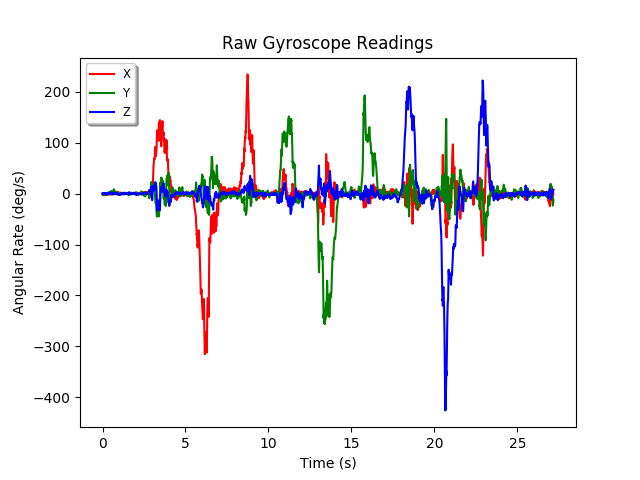
\includegraphics[width=.32\textwidth]{gyro-unaltered}\hfill
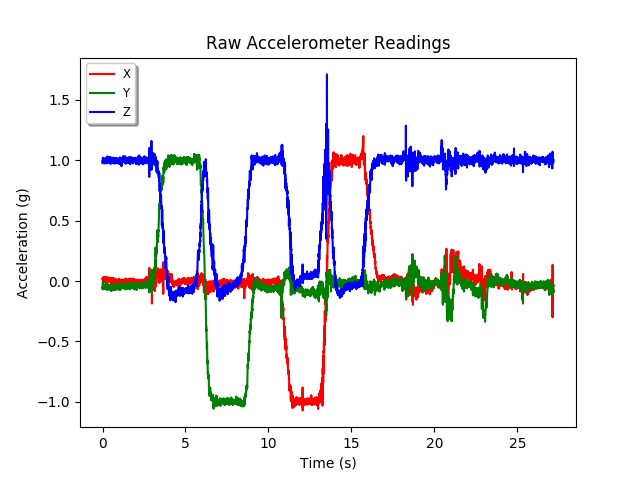
\includegraphics[width=.32\textwidth]{acc-unaltered}\hfill
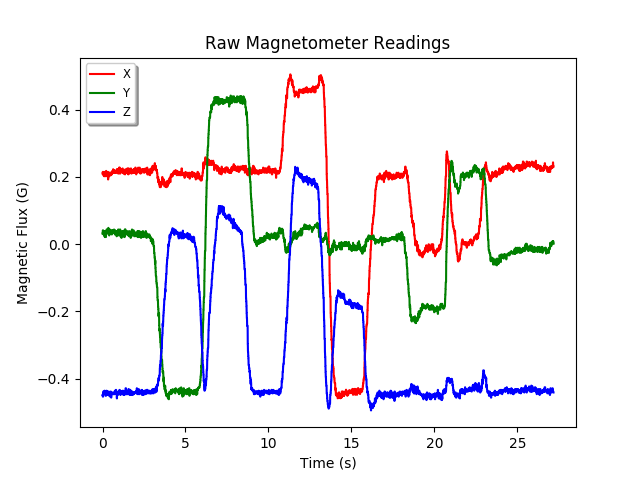
\includegraphics[width=.32\textwidth]{mag-unaltered}

\caption{Raw sensor readings from the IMU. Raw accelerometer data clearly displaying the $z$-axis as the initial `up' position, so tilt corrections are made towards this axis, yaw corrections are made around this axis.}
\label{fig:raw-readings}

\end{figure}

\begin{figure}[htp]

\centering
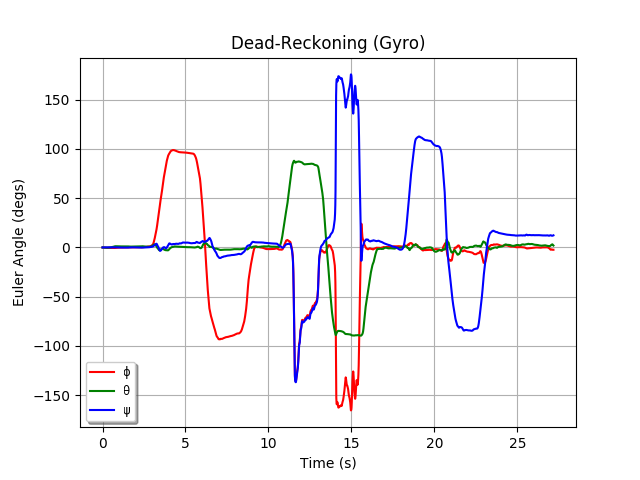
\includegraphics[width=.32\textwidth]{1gyro_dead}\hfill
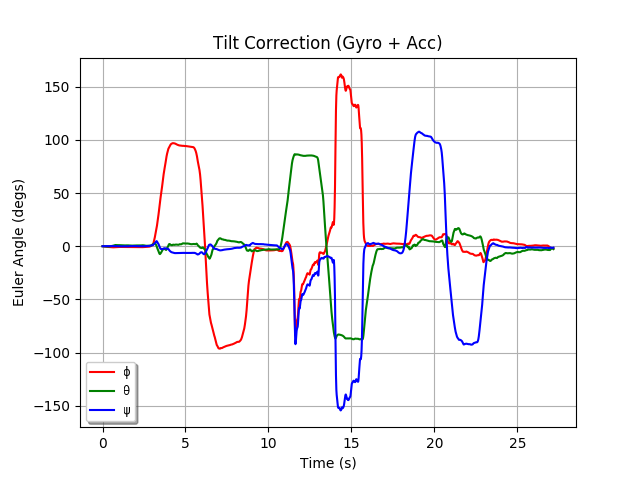
\includegraphics[width=.32\textwidth]{2gyro_acc}\hfill
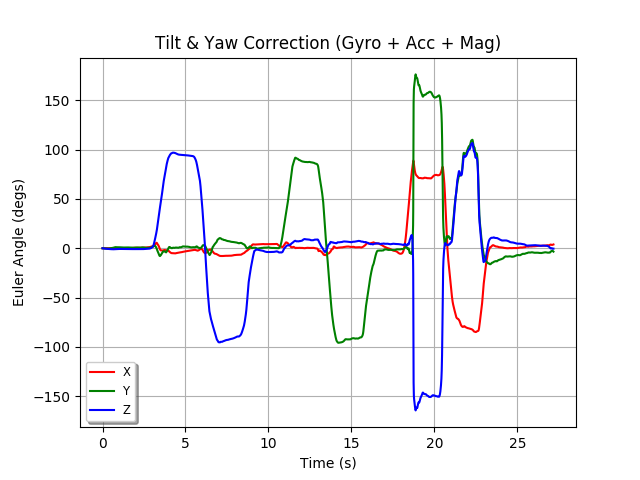
\includegraphics[width=.32\textwidth]{3gyro_acc_mag}

\caption{Euler angle readings, with and without various levels of correction. For tilt correction, $\alpha_{tilt}=0.01$. For tilt \& yaw correction, $\alpha_{tilt}=0.1$, $\alpha_{yaw}=0.001$. Notice the clear improvements and reduction in axis drift as more levels of error correction are added to the raw dead reckoning data.}
\label{fig:euler-angles}

\end{figure}



\end{document}